\begin{figure*}
    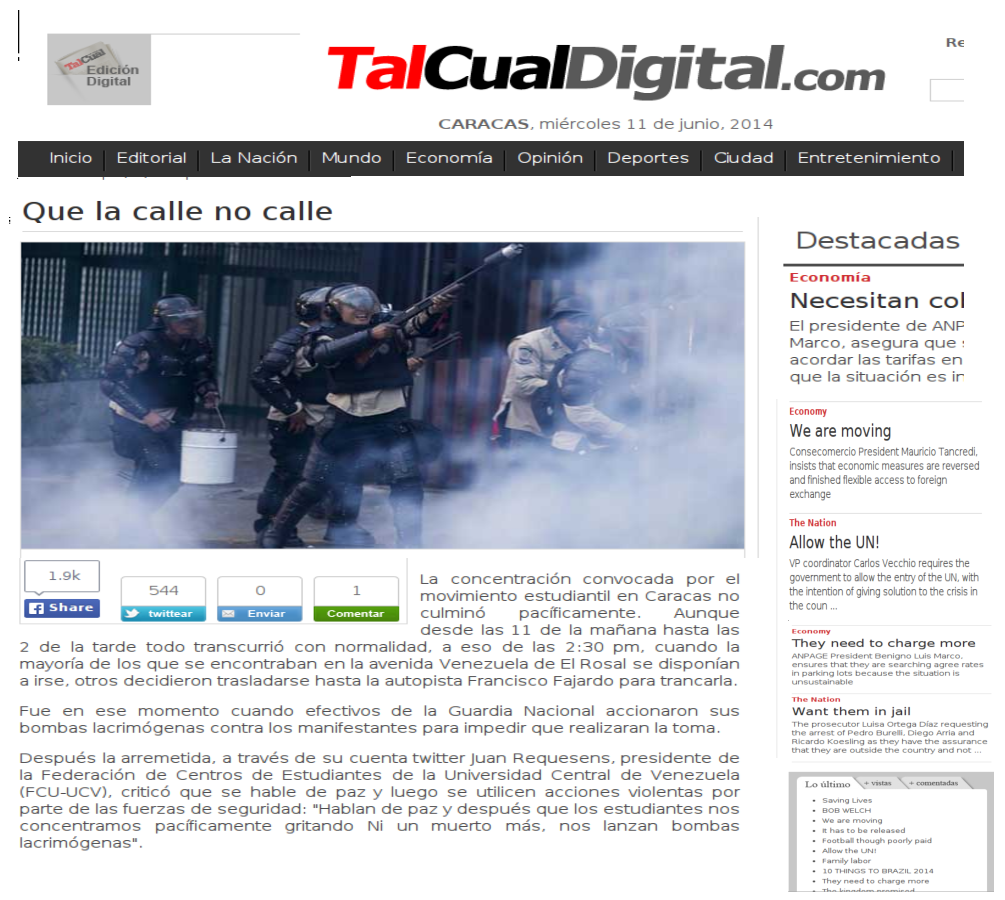
\includegraphics[width=0.5\textwidth, height=0.4\textwidth]{pp_example}
    \caption{An example of a planned protest article}
    \label{pp_example}
\end{figure*}
Civil unrest (protests, strikes, and ``occupy'' events) is a common happening in both democracies
and authoritarian regimes.
Although we typically associate civil unrest with disruptions and instability, for a social scientist
civil unrest reflects the democratic process by 
which citizenry communicate their views and preferences to those in authority. 
The advent of social
media has afforded citizenry new mechanisms for organization and mobilization, and online news sources
and social networking sites like Facebook and Twitter
can provide a window into civil unrest happenings in a particular country.

Our basic hypothesis is that
protests that are larger will be more disruptive and communicate support for its cause better than smaller protests. 
Mobilizing large numbers of people is more likely to occur if a protest is organized and the time and place announced in
advance. Because protest is costly and more likely to succeed if it is large, we should expect planned, rather than 
spontaneous, protests to be the norm. Indeed, in a sample of 288 events from our study selected for qualitative review of their antecedents
(more details later), for 225 we located communications regarding the upcoming occurrence of the event in media, and only 49 were classified as 
spontaneous (we could not determine whether communications had or had not occurred in the remaining 14 cases).

\narenc{fix this text after Sathappan adds a figure.}
Our goal here thus is to develop a protest forecasting system by identifying and mining mentions of future planned events
in (news and social) media. Why is this problem difficult? Consider the following situation:
\begin{quote}
An article is published in {\it El Universal}
in {\it Caracas, Venezuela} about a protest that happened over the {\it Friendship bridge} in {\it Foz do Iguacu, Brazil} due to
some conflict with citizens of {\it Paraguay}
across the border.
\end{quote}


We sought to develop
computational techniques for detecting overt direct indicators
of upcoming planned civil unrest events automatically from openly
available sources of information.  Detecting indicators for civil
unrest planning activities might have application to a wide range of
governmental and civil activity, from the issuance of travel warnings
to rapid emergency response capabilities.  
Our detection approach 
combine shallow linguistic analysis to identify a corpus of relevant
documents (articles, tweets) which are then subject to targeted deep semantic analysis.
Despite its simplicity, we are able to
detect indicators of event planning with surprisingly high
accuracy. 
Our contributions are:
\begin{enumerate}
\item We present a protest forecasting system that couples three key technical ideas:
key phrase learning to identify what to look for, probabilistic soft logic to reason about location occurrences in extracted results, and 
time normalization to resolve future tense mentions. We demonstrate how the integration of these ideas achieves objectives in precision,
recall, and quality (accuracy).
\item We illustrate the application of our system to 10 countries in Latin America, viz. Argentina, Brazil, Chile, Colombia, Ecuador, El Salvador, Mexico, Paraguay, Uruguay, and Venezuela. 
We conduct ablation studies to identify the 
relative contributions of news media (news + blogs) versus social media (Twitter, Facebook) to identify future happenings of
civil unrest. Through these studies we illustrate the selective superiorities of different sources for specific countries.
\narenc{Graham said to give some numerical values here.}
\item Unlike many studies of retrospective forecasting of protests,
we assess the lead time from when the forecast is made to
the actual event date, to assess the forecasting prowess of our approach. 
Our results demonstrate that we are able to 
capture significant societal unrest in the above countries with an average lead time of 4.08 days. This illustrates that the
approach here can be used in a practical protest forecasting system.
\end{enumerate}

